\documentclass[12pt]{exam}

\usepackage{setspace}
\setstretch{1.15}
\nopointsinmargin
\pointformat{}

\usepackage{problemset}
\usepackage[margin=1in]{geometry}

\noprintanswers
%\printanswers

\begin{document}

\FontEasyRead

\newcommand{\entryblank}{\raisebox{0.4ex}{\rule{0.4cm}{0.6pt}}}

\Heading
{Microeconomics}
{Test on Chapters 1--4, 6--9}
{75 Minutes, 100 points.
  Open book, notes, computer, and annotated cheat-sheet permitted.
  Calculator recommended.
  Answer all questions. Show all work for math problems.
Do not skip any problems---there is always potential for partial credit.}

\begin{questions}

  %%%%%%%%%%%%%%%%%%%%%%%%%%%%%%%%%%%%%%%%%%%%%%%%%%%%%%
  \section*{Problems}

  \begin{problem}[15]{4in}
    Assuming typical supply and demand curves, fill in each box with the effect on
    equilibrium price and quantity. Uses these codes:

    \begin{itemize}
      \item Price up, same, down, ambiguous: P-U, P-S, P-D, P-A
      \item Quantity up, same, down, ambiguous:  Q-U, Q-S, Q-D, Q-A
    \end{itemize}

    ``Ambiguous'' means the outcome could be up, same, or down, depending on the
    relative magnitudes and/or elasticities.

    \vspace{0.5cm}

    \begin{center}
      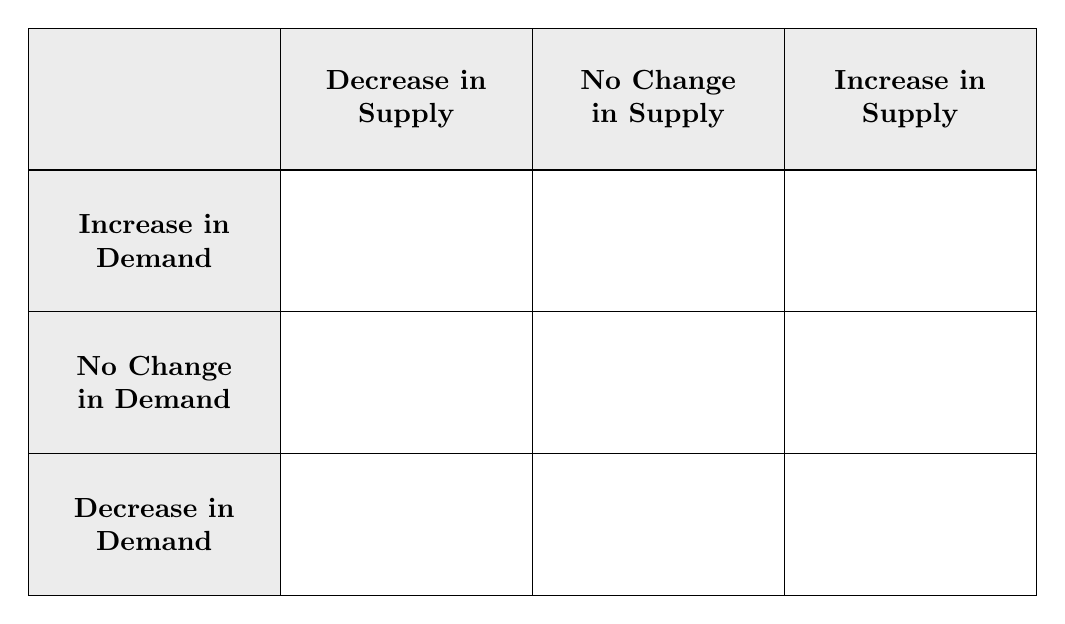
\begin{tikzpicture}[
          every node/.style={draw, align=center, minimum height=1.8cm},
          header/.style={font=\bfseries, fill=gray!15},
          cell/.style={minimum width=3.2cm},
          rowlabel/.style={minimum width=3.2cm, font=\bfseries, fill=gray!15}
        ]

        % Top row (column headers)
        \node[header, minimum width=3.2cm] at (0,0) {};
        \node[header, cell] at (3.2,0) {Decrease in\\Supply};
        \node[header, cell] at (6.4,0) {No Change\\in Supply};
        \node[header, cell] at (9.6,0) {Increase in\\Supply};

        % Row 1
        \node[rowlabel] at (0,-1.8) {Increase in\\Demand};
        \node[cell] at (3.2,-1.8) {};
        \node[cell] at (6.4,-1.8) {};
        \node[cell] at (9.6,-1.8) {};

        % Row 2
        \node[rowlabel] at (0,-3.6) {No Change\\in Demand};
        \node[cell] at (3.2,-3.6) {};
        \node[cell] at (6.4,-3.6) {};
        \node[cell] at (9.6,-3.6) {};

        % Row 3
        \node[rowlabel] at (0,-5.4) {Decrease in\\Demand};
        \node[cell] at (3.2,-5.4) {};
        \node[cell] at (6.4,-5.4) {};
        \node[cell] at (9.6,-5.4) {};

      \end{tikzpicture}
    \end{center}

    Sketch here as needed to help you:

  \end{problem}

  %%%%%%%%%%%%%%%%%%%%%%%%%%%%%%%%%%%%%%%%%%%%%%%%%%%%%%

  \begin{shortanswer}[10]{2.5in}
    A sudden 25\% increase in the price of refrigerators causes quantity
    demanded to fall sharply at first, but later recover. Explain what's happening
    in terms of short-run and long-run price elasticity of demand.  Are refrigerators
    durable or non-durable goods?
  \end{shortanswer}

  \begin{solution}
    Short-run demand is more elastic (consumers make-do with their old refrigerators); long-run
    demand is more inelastic as consumers adjust (and their old fridges wear out). Refrigerators
    are durable goods.
  \end{solution}

  %%%%%%%%%%%%%%%%%%%%%%%%%%%%%%%%%%%%%%%%%%%%%%%%%%%%%%

  \begin{problem}[15]{3in}
    Given the CPI-U table:

    \begin{center}
      \renewcommand{\arraystretch}{1.4}
      \setlength{\tabcolsep}{12pt}

      \begin{tabular}{|>{\centering\arraybackslash}p{3cm}|>{\centering\arraybackslash}p{5cm}|}
        \hline
        \textbf{Year} & \textbf{CPI-U Annual Average Index} \\
        \textbf{} & \textbf{(1982--1984 = 100)} \\
        \hline
        2020 & 258.811 \\
        \hline
        2021 & \entryblank \\
        \hline
        2022 & 292.655 \\
        \hline
        2023 & \entryblank \\
        \hline
        2024 & 319.799 \\
        \hline
      \end{tabular}
    \end{center}

    Given:
    \begin{itemize}
      \item Inflation from 2020 to 2021 = 4.69802\%
      \item Average annual inflation from 2020 to 2023 = 5.76852\%
    \end{itemize}

    Find the missing CPI values.
  \end{problem}
  \begin{solution}
    Apply inflation formula:
    \[
      CPI_{2021} = 258.811 \times (1.0469802)
    \]
    and compound for 2023.
  \end{solution}

  %%%%%%%%%%%%%%%%%%%%%%%%%%%%%%%%%%%%%%%%%%%%%%%%%%%%%%

  \begin{problem}[10]{2.5in}
    Demand: \( Q_d = 100 - 2P \) \\
    Supply: \( Q_s = 3P + 10 \)

    The government sets \( P = 20 \).

    Find:
    \begin{itemize}
      \item Quantity demanded
      \item Quantity supplied
      \item Size and type of disequilibrium
    \end{itemize}
  \end{problem}

  \begin{solution}
    Compute:
    \[
      Q_d = 100 - 40 = 60, \quad Q_s = 70
    \]
    Surplus of 10 units.
  \end{solution}

  %%%%%%%%%%%%%%%%%%%%%%%%%%%%%%%%%%%%%%%%%%%%%%%%%%%%%%

  \begin{problem}[10]{2in}
    Classify each as Positive (P) or Normative (N):

    \begin{enumerate}
      \item A monopoly sets higher prices than in perfect competition.
      \item Healthcare should be free to all.
      \item Minimum wage increases unemployment.
      \item Rent control is the fairest policy.
      \item Socialized medicine provides best outcomes.
    \end{enumerate}
  \end{problem}

  \begin{solution}
    P, N, P, N, N
  \end{solution}

  %%%%%%%%%%%%%%%%%%%%%%%%%%%%%%%%%%%%%%%%%%%%%%%%%%%%%%

  \begin{shortanswer}[5]{2in}
    Explain the difference between:
    \begin{itemize}
      \item Increase in demand
      \item Increase in quantity demanded
    \end{itemize}
    Give an example of each.
  \end{shortanswer}

  \begin{solution}
    Demand shift vs movement along curve.
  \end{solution}

  %%%%%%%%%%%%%%%%%%%%%%%%%%%%%%%%%%%%%%%%%%%%%%%%%%%%%%

  \begin{problem}[15]{4in}
    Given:
    \[
      MR(q) = 100 - 4q, \quad MC(q) = 20 + q
    \]

    \begin{itemize}
      \item Find profit-maximizing \( q \)
      \item Find price using \( P(q) = 100 - 2q \)
      \item Find total revenue
      \item Given \( C(q) = 20q + 0.5q^2 \), compute profit
    \end{itemize}
  \end{problem}

  \begin{solution}
    Set \( MR = MC \):
    \[
      100 - 4q = 20 + q \Rightarrow q = 16
    \]
    \[
      P = 100 - 32 = 68
    \]
    \[
      TR = 68 \cdot 16 = 1088
    \]
    \[
      C = 320 + 128 = 448
    \]
    Profit = 640
  \end{solution}

  %%%%%%%%%%%%%%%%%%%%%%%%%%%%%%%%%%%%%%%%%%%%%%%%%%%%%%

  \begin{problem}[20]{5in}
    Production function:
    \[
      Q = L^{0.5}K^{0.5}
    \]

    Given:
    \[
      w = 10, \quad r = 20, \quad Q = 100
    \]

    \begin{itemize}
      \item Find MPL and MPK
      \item Use cost minimization condition:
        \[
          \frac{MPL}{MPK} = \frac{w}{r}
        \]
        to express \( K \) as a function of \( L \)
      \item Solve for optimal \( L \) and \( K \)
    \end{itemize}
  \end{problem}

  \begin{solution}
    \[
      MPL = 0.5L^{-0.5}K^{0.5}, \quad MPK = 0.5L^{0.5}K^{-0.5}
    \]
    \[
      \frac{MPL}{MPK} = \frac{K}{L} = \frac{w}{r} = \frac{1}{2}
      \Rightarrow K = \frac{L}{2}
    \]
    Substitute:
    \[
      100 = \sqrt{L \cdot \frac{L}{2}} = \frac{L}{\sqrt{2}}
      \Rightarrow L \approx 141.4, \quad K \approx 70.7
    \]
  \end{solution}

  %%%%%%%%%%%%%%%%%%%%%%%%%%%%%%%%%%%%%%%%%%%%%%%%%%%%%%

\end{questions}

\end{document}
